% Document class
\documentclass[12pt,a4paper]{article}

% Required Packages
\usepackage{amsmath, url}
\usepackage[francais]{babel}
\usepackage{fontspec}
\usepackage{color}
\usepackage{color,xcolor,ucs,soul}
\usepackage{sectsty}
\usepackage{hyperref, tikz}
\usepackage{eso-pic, titlesec, fancyhdr, fancyvrb}
\usepackage{multicol}
\usepackage{fancyvrb}
\usepackage{abstract}
\usepackage{listings}
\usepackage{framed,graphicx,xcolor}

\definecolor{shadecolor}{rgb}{1,0,0}

\providecommand{\tightlist}{%
  \setlength{\itemsep}{0pt}\setlength{\parskip}{0pt}}


% Configuration colors
\definecolor{dcblue}{HTML}{3A619B}
\definecolor{dcyellow}{HTML}{F4DD19}
\definecolor{dcbluelight}{HTML}{709EA4}
\definecolor{dcbluealt}{HTML}{25415E}
\definecolor{dcbluecover}{HTML}{335F93}
\definecolor{dcbluetext}{HTML}{002C5C}

% Font properties
\setmainfont{Gotham}
\defaultfontfeatures{Ligatures=TeX}
\AtBeginDocument{\color{dcbluetext}}
\partfont{\color{dcbluelight}}
\sectionfont{\color{dcbluelight}}
\subsectionfont{\color{dcbluelight}}
\subsubsectionfont{\color{dcbluelight}}

% Default commands

\newcommand{\twocols}[1]{
  \begin{multicols}{2}
    #1
  \end{multicols}
}

\fancyhead[R]{\bfseries\color{dcbluealt}\nouppercase\leftmark}
\fancyhead[L]{}
\renewcommand{\headrulewidth}{1.5pt}
\renewcommand{\headrule}{{\color{dcyellow}
\hrule width\headwidth height\headrulewidth \vskip-\headrulewidth}}
\fancyfoot[C]{\bfseries\color{dcbluelight}\thepage}

\newcommand{\VerbBar}{|}
\newcommand{\VERB}{\Verb[commandchars=\\\{\}]}
\DefineVerbatimEnvironment{Highlighting}{Verbatim}{commandchars=\\\{\}}
% Add ',fontsize=\small' for more characters per line
\newenvironment{Shaded}{}{}
\newcommand{\KeywordTok}[1]{\textcolor[rgb]{0.00,0.44,0.13}{\textbf{{#1}}}}
\newcommand{\DataTypeTok}[1]{\textcolor[rgb]{0.56,0.13,0.00}{{#1}}}
\newcommand{\DecValTok}[1]{\textcolor[rgb]{0.25,0.63,0.44}{{#1}}}
\newcommand{\BaseNTok}[1]{\textcolor[rgb]{0.25,0.63,0.44}{{#1}}}
\newcommand{\FloatTok}[1]{\textcolor[rgb]{0.25,0.63,0.44}{{#1}}}
\newcommand{\ConstantTok}[1]{\textcolor[rgb]{0.53,0.00,0.00}{{#1}}}
\newcommand{\CharTok}[1]{\textcolor[rgb]{0.25,0.44,0.63}{{#1}}}
\newcommand{\SpecialCharTok}[1]{\textcolor[rgb]{0.25,0.44,0.63}{{#1}}}
\newcommand{\StringTok}[1]{\textcolor[rgb]{0.25,0.44,0.63}{{#1}}}
\newcommand{\VerbatimStringTok}[1]{\textcolor[rgb]{0.25,0.44,0.63}{{#1}}}
\newcommand{\SpecialStringTok}[1]{\textcolor[rgb]{0.73,0.40,0.53}{{#1}}}
\newcommand{\ImportTok}[1]{{#1}}
\newcommand{\CommentTok}[1]{\textcolor[rgb]{0.38,0.63,0.69}{\textit{{#1}}}}
\newcommand{\DocumentationTok}[1]{\textcolor[rgb]{0.73,0.13,0.13}{\textit{{#1}}}}
\newcommand{\AnnotationTok}[1]{\textcolor[rgb]{0.38,0.63,0.69}{\textbf{\textit{{#1}}}}}
\newcommand{\CommentVarTok}[1]{\textcolor[rgb]{0.38,0.63,0.69}{\textbf{\textit{{#1}}}}}
\newcommand{\OtherTok}[1]{\textcolor[rgb]{0.00,0.44,0.13}{{#1}}}
\newcommand{\FunctionTok}[1]{\textcolor[rgb]{0.02,0.16,0.49}{{#1}}}
\newcommand{\VariableTok}[1]{\textcolor[rgb]{0.10,0.09,0.49}{{#1}}}
\newcommand{\ControlFlowTok}[1]{\textcolor[rgb]{0.00,0.44,0.13}{\textbf{{#1}}}}
\newcommand{\OperatorTok}[1]{\textcolor[rgb]{0.40,0.40,0.40}{{#1}}}
\newcommand{\BuiltInTok}[1]{{#1}}
\newcommand{\ExtensionTok}[1]{{#1}}
\newcommand{\PreprocessorTok}[1]{\textcolor[rgb]{0.74,0.48,0.00}{{#1}}}
\newcommand{\AttributeTok}[1]{\textcolor[rgb]{0.49,0.56,0.16}{{#1}}}
\newcommand{\RegionMarkerTok}[1]{{#1}}
\newcommand{\InformationTok}[1]{\textcolor[rgb]{0.38,0.63,0.69}{\textbf{\textit{{#1}}}}}
\newcommand{\WarningTok}[1]{\textcolor[rgb]{0.38,0.63,0.69}{\textbf{\textit{{#1}}}}}
\newcommand{\AlertTok}[1]{\textcolor[rgb]{1.00,0.00,0.00}{\textbf{{#1}}}}
\newcommand{\ErrorTok}[1]{\textcolor[rgb]{1.00,0.00,0.00}{\textbf{{#1}}}}
\newcommand{\NormalTok}[1]{{#1}}
\usepackage{graphicx,grffile}


% Document meta
\title{Rapport de stage TN09: Dveloppement d'applications web en React et Redux}
\author{Aurélie \bsc{Digeon}}

% Document
\begin{document}

  {
    \begin{titlepage}
      \makeatletter
      \begin{tikzpicture}[
          overlay,
          remember picture,
          anchor=north west,
          inner sep=0pt,
          outer sep=0pt,
          fill opacity=.74
        ]
        \node[inner sep=0] at (current page.north west)
        {\includegraphics[height=\pdfpageheight]{layout/cover.jpg}};
        \draw[fill=dcbluecover]
          (current page.north west) rectangle (current page.south east);
      \end{tikzpicture}

      \begin{center}
        {\fontspec{Omnes}
          {\Huge {\textcolor{dcyellow}{\textbf{
            {\MakeUppercase{\@title}}
          }}\par}}
        }
        \vskip 2em
        {\large
        \begin{tabular}[t]{c}
          {\textcolor{white}{\@author}}
        \end{tabular}
        \par}
      \end{center}

      \vfill

      \begin{center}
        {
\includegraphics[width=5cm]{layout/logo.png}}
      \end{center}
      \begin{center}
        {
\includegraphics[width=3cm]{layout/logosUTC_SUnb.png}}
      \end{center}
      \makeatother
    \end{titlepage}
    \thispagestyle{empty}
    \tableofcontents
    \newpage
  }


  \pagestyle{fancy}
  %% start writing here

  \newpage

  \section{Remerciements}\label{remerciements}

  \bigskip

  Je tiens tout d'abord à remercier Benjamin Tierny, Robin Komiwes et
  Julien Vanden Torren pour m'avoir acceuilli chez Dernier Cri, pour mon
  stage.

  \bigskip

  Je remercie également mon suiveur Harry Claisse pour son aide et son
  accompagnement, ainsi que les enseignants de l'Université de
  Technologiques de Compiègne.

  \bigskip

  Merci également à toute l'équipe de Dernier cri pour avoir rendu mon
  stage enrichissant et agréable, et pour m'avoir accueuilli à bras
  ouverts.

  \bigskip

  J'aimerai finalement remercier mes parents et mon frère, qui m'ont
  permis de faire ces études et m'ont soutenu durant ce stage.

  \newpage

  \iffalse
  \# Résumé et abstract

  \bigskip

  \subsection{Résumé}\label{ruxe9sumuxe9}

  \newpage

  \subsection{Abstract}\label{abstract}

  \newpage

  \fi

  \section{Introduction}\label{introduction}

  \bigskip

  Dans le cadre de mon stage de TN09, lors de ma quatrième année
  d'ingénieur en informatique à l'Université de Technologique de Compiègne
  (UTC), j'ai effectué un stage de six mois chez Dernier cri.

  \bigskip

  Dernier Cri est une \emph{start-up} créée en 2011, spécialisée dans
  l'innovation numérique. L'équipe est en charge du développement, du
  déploiement et de la maintenance d'applications pour le compte de
  plusieurs clients.

  \bigskip

  Ma mission a été d'intégrer l'équipe de développement pour aider dans la
  création de plusieurs applications web.

  \bigskip

  J'ai pu, lors de ce stage, intégrer une équipe dynamique et pro-active.
  En plus de mon implications dans les projets pour des clients, j'ai pu
  prendre part à de nombreuses présentations internes sur différentes
  technologies, et à l'écriture d'articles de blog. J'ai également pu
  participer activement à la relation client lors de mes projets.

  \bigskip

  Dans ce rapport je vais vous présenter tout d'abord Dernier cri,
  l'entreprise qui m'a accueilli. Je vous exposerais les techniques de
  travail et les différents moyens de s'exprimer qu'elle offre à ses
  équipes.

  \bigskip

  Je vous exposerai ensuite ma mission au sein de l'entreprise. Je
  détaillerai les technologies que j'ai utilisé mais aussi la gestion de
  projet ainsi que la relation client, qui sont des éléments clés dans la
  bonne conduite d'un projet.

  \bigskip

  Finalement, il me tient à coeur de présenter la communauté de Lille et
  ses particularités. En effet, le dynamisme de la communauté et la
  diversité des événements proposés m'ont beaucoup aidé à m'intégrer et à
  approfondir mon projet professionnel.

  \newpage

  \section{Dernier cri}\label{dernier-cri}

  \bigskip

  \subsection{Histoire}\label{histoire}

  \bigskip

  En 2011, Robin Komiwes et Benjamin Tierny créent Nectify, une entreprise
  dont le but est le développement et la commercialisation de Fresc, un
  outil de partage d'avis sur des visuels. Bien que cet outil connaîtra un
  succès mérité (on comptabilise aujourd'hui près de 300 entreprises
  l'utilisant à travers de milliers de projets), la rentabilité financière
  n'est pas suffisante pour assurer la pérennité de l'entreprise.

  \bigskip

  Nectify choisit alors de compléter ses revenus par de la prestation de
  services centrés sur l'innovation.

  \bigskip

  Début 2014, la majeure partie du chiffre d'affaire de Nectify était dû
  aux activités de prestations de services, Fresc ne représentant qu'une
  part marginale.

  \bigskip

  Devenant donc une agence spécialisée dans l'innovation digitale, Nectify
  choisit de créer sa propre image, distincte de Fresc. C'est dans ce
  mouvement que la société est devenue Dernier cri.

  \bigskip

  Aujourd'hui, Dernier cri est une agence web qui met un point d'honneur à
  proposer à ses clients une solution complète et adaptée à leur
  problèmatique. De la conception à la réalisation, l'entreprise
  accompagne ses clients de A à Z pour aboutir à un produit au plus proche
  de leurs besoins. Cela permet aux développeurs d'opérer dans différents
  domaines d'activités, et d'avoir une vue globale du développement du
  produit.

  \bigskip

  \subsection{Secteur d'activité}\label{secteur-dactivituxe9}

  \bigskip

  Le secteur de l'informatique est aujourd'hui est en pleine expension et
  ne connait pas la crise. Pour donner un ordre d'idée, le marché de la
  programmation et des services informatiques embauche près de 400 000
  personnes dans ses 21 000 ESN (Entreprises de Services du Numérique) et
  ne cesse de croître depuis ces cinq dernières années.

  \bigskip

  Dernier cri est une \emph{start-up} spécialisée dans l'innovation
  digitale. Elle se démarque notamment des autres agences web en proposant
  plusieurs services, dont évidemment la création d'applications
  web/mobile, mais aussi l'application de la recherche fondamentale en
  apprentissage automatique et traitement de gros volumes de données, afin
  d'augmenter la capacité d'innovation d'entreprises tiers. Cela se
  traduit notamment par de l'exploration de connaissances à partir de
  données pour des magasins, par exemple, ou la création d'audit.

  \bigskip

  C'est cette diversité qui permet à Dernier cri de se démarquer dans
  l'univers du web à Lille, où de nombreuse agences se partagent le
  marché.

  \bigskip

  \subsection{Organisation}\label{organisation}

  \bigskip

  Dernier cri est une entreprise à taille humaine. Cela se traduit par des
  cycles de décision courts, des dirigeants plus accessibles et la volonté
  de travailler dans un esprit d'équipe.

  \bigskip

  Dernier cri posséde une organisation souple qui offre l'opportunité à
  tous de s'impliquer dans les projets, que ce soit pour des clients ou
  bien en interne.

  \bigskip

  Au sommet de l'organisation de l'entreprise se trouve les deux
  fondateurs ainsi que le troisième associé. Le directeur général de
  l'entreprise (CTO) est Benjamin Tierny, tandis que Robin Komiwes est le
  directeur de la technologie (CTO). Le troisième associé, Julien Vanden
  Torren, est Account Manager, c'est à dire le lien entre l'entreprise et
  les clients.

  \bigskip

  L'entreprise compte aujourd'hui 18 employés mais se trouve dans une
  phase d'expension avec de nouvelles embauches en perspective, grace à de
  nombreux nouveaux projets.

  \bigskip

  L'équipe est également constituée d'une chef de projet, Laetitia
  Cocusse, qui s'occupe de superviser la plupart des projets.

  \bigskip

  Dernier Cri est à la fois une agence Web mais aussi une agence qui se
  préoccupe des problèmes actuels liés à l'ingénierie système et au
  traitement de grosses données. C'ets pourquoi l'équipe de développeurs
  est aussi constituée d'un \emph{devops}, c'est à dire d'une personne
  possédant à la fois les compétences d'un développeur et d'un ingénieur
  système, d'un \emph{Data Scientist} qui travaille sur les projets de big
  data.

  \bigskip

  La plupart des développeurs travaille sur plusieurs projets en même
  temps, selon les besoins de l'entreprise et les compétences de chacun.
  Des équipes de 2/3 développeurs sont crées, mélangeant les compétences
  \emph{front} et \emph{back}, de développement et de système.

  \bigskip

  TODO gestion de projet, github

  \bigskip

  Dernier Cri a à coeur de développer une culture entreprenariale et
  informatique, c'est pourquoi s'est developpé des présentations internes
  (dont certaines sont diffusées via une chaine youtube) ainsi que des
  présentations publiques par l'intermédiaire de \emph{blog posts} .

  \subsubsection{Talk interne}\label{talk-interne}

  \bigskip

  Dans l'optique d'un partage du savoir dans l'entreprise, les employés
  sont invités à faire des \emph{talks}, c'est-à-dire de petites
  présentations. Celles-ci ont pour objectif de présenter certains enjeux
  et solutions techniques en rapport avec la réalisation d'un projet, le
  résultat d'une veille, ou tout simplement un sujet qui les intéresse.
  Les \emph{talks} techniques permettent aux membres d'une équipe de
  partager entre eux leurs expériences et leurs passions.

  \bigskip

  Ces présentations ont deux principaux avantages. Tout d'abord elles
  permettent aux spectateurs de la présentation d'apprendre de nouvelles
  choses. C'est l'occasion de découvrir un sujet dont on ne se doutait pas
  de l'intéret ou bien de l'existence. De plus, la présentation est
  travaillée et structurée, car une personne a déjà fait l'effort de trier
  les informations et de les présenter de la manière la plus lisible,
  claire, et/ou ludique. C'est ainsi souvent beaucoup plus facile
  d'aborder un sujet avec ces \emph{talks}, que de devoir effectuer une
  recherche d'information sur divers supports.

  \bigskip

  Le second avantage concerne l'organisateur de la présentation. Tout
  d'abord, sensibiliser ses coéquipiers à des problèmes, ou des
  technologies, peut être un véritable gain de temps pour le futur. En
  effet, cela permet de mutualiser la communication, et d'éviter de devoir
  expliquer individuellement les concepts.

  \bigskip

  De plus, l'organisateur apprend beaucoup car, pour la création de la
  présentation, il doit devenir un expert sur le sujet qu'il va couvrir.
  Il devra assez approfondir le sujet pour être capable, d'une part d'être
  clair dans sa présentation, d'autre part de répondre aux éventuelles
  questions. Pour lui c'est aussi une occasion de travailler sur ces
  compétences d'orateur. Cela peut évidemment lui être utile pour son
  travail, sa vie de tout les jours, mais surtout un \emph{talk} interne
  peut faire office d'incubation pour une présentation dans un autre
  contexte. En effet, il existe à Lille de nombreux évènements où il est
  possible de faire des présentations, ce qui est très intéréssant mais
  aussi peut être assez intimidant. Le présentateur peut tester son talk
  en interne avant d'en faire partager la communauté.

  \bigskip

  Finalement, présenter un sujet issu d'une veille technologique permet,
  au-delà de faire découvrir aux autres un sujet potentiellement
  intéressant, de certifier l'intérêt du sujet. En effet, beaucoup de
  sujets qui semblent prometteur peuvent, avec un peu de recherche, se
  révéler creux et sans intêret.

  \bigskip

  Les \emph{talks} internes sont aussi une très bonne manière de partager
  des connaissances de manière ludique. Durant mon stage j'ai eu
  l'occasion d'assister à des présentations sur de nombreuses technologies
  telles que \emph{React}, \emph{Docker}, \emph{Rust}, \emph{MJML}\ldots{}
  Mais aussi sur des sujets variés comme le Growth hacking (Ensemble de
  techniques de marketing permettant d'accélérer rapidement et
  significativement la croissance d'une \emph{start-up}.), ou encore la
  fabrication d'un audit.. Ces présentations sont publiées sur la
  \href{https://www.youtube.com/channel/UCDfdBlzldhg_PEu3xZTPsHg}{chaîne
  youtube Dernier cri}. Cela m'a permis de découvrir de nouveaux sujets et
  de mieux comprendre les discutions, et les problématiques que
  rencontraient mes collègues.

  \bigskip

  \subsubsection{Article de blog}\label{article-de-blog}

  \bigskip

  Dernier Cri posséde également un
  \href{http://derniercri.io/tech-blog}{blog technique} alimenté par les
  développeurs de l'équipe. Les objectifs sont notablement les mêmes que
  pour les présentations internes. Mais cela permet aussi à Dernier cri de
  rayonner et montrer ses compétences techniques et son esprit d'analyse.

  \bigskip

  Le blog technique permet à Dernier Cri de se positionner en tant
  qu'expert. Publier des articles blog est excellent pour la réputation.
  En délivrant des conseils professionnels utiles, Dernier Cri prouve sa
  maîtrise de son activité.

  \bigskip

  Cela permet également d'améliorer la visibilité de l'entreprise en
  exposant son savoir et savoir-faire à une large communauté
  professionnelle. Un blog est également utile pour tenir informée sa
  communauté : il permet de rester en contact permanent avec ses prospects
  et de les tenir au courant de toute l'actualité de son entreprise, comme
  un nouveau produit, une nouvelle technologie maitrisée \ldots{}

  \bigskip

  Pour le rédacteur de l'article, cela a également de nombreux avantages.
  Par exemple, cela lui permet de travailler sa rédaction et son
  argumentation, de partager avec d'autres développeurs à travers les
  commentaires, de gagner en visibilité et en réputation, ou encore de se
  forcer à rester à la page, pour être exhaustif et à jour dans ses
  références.

  \bigskip

  J'ai moi-même eu l'occasion lors de mon stage d'écrire un article pour
  le blog technique de Dernier cri. Dans cet article je décris les
  technologies que j'ai utilisé lors de mon stage, React et Redux, ainsi
  que cinq outils que j'ai découvert et qui m'ont facilité la vie pour
  utiliser ses technologies. Ce fut une expérience très enrichissante.
  Cela m'a poussé à enrichir mes connaissances dans le domaine, de
  clarifier les concepts pour savoir les expliquer à tous et de travailler
  ma qualité de rédaction.

  \newpage

  \section{Cadre du stage}\label{cadre-du-stage}

  \bigskip

  Durant mon stage j'ai rejoint l'équipe de développeurs de l'entreprise
  et j'ai pu participer au développement de deux applications. Ces deux
  projets s'appuyaient sur le framework ReactJS, une bibliothèque
  JavaScript open-source développée par Facebook depuis 2013. N'ayant
  jamais utilisé cette bibliothèque, j'ai donc du tout d'abord me former.

  \bigskip

  Le premier projet auquel j'ai participé se nomme Photolix. C'est un site
  internet de développement de photos, avec pour objectifs de toucher un
  large public et de limiter au maximum le temps d'attente du client en
  envoyant les photos au serveur dès leur sélection.

  \bigskip

  Le second projet est FinFrog, un site proposant des prêts financés par
  des particuliers. Ce projet était déjà assez avancé à mon arrivé. Le
  client possédait un site en ligne, mais souhaitait changer l'apparence
  et ajouter des fonctionnalités, ce pourquoi il a fait appel à Dernier
  cri.

  \bigskip

  \subsection{Formation}\label{formation}

  \bigskip

  Lors de mon arrivée chez Dernier cri, j'ai eu l'occasion de me former
  sur Javascript ES6, React ainsi que Redux, car l'entreprise prévoyait de
  me mettre sur des projets utilisant ces technologies.

  \bigskip

  La popularité de ces trois technologies est en forte hausse, et de plus
  en plus demandée et utilisée pour la création d'applications web. C'est
  pourquoi ce fut une véritable chance d'apprendre ces deux frameworks
  lors de mon stage.

  \bigskip

  Ma formation s'est faite à partir du site
  \href{https://www.codeschool.com/}{Code school}, disposant de cours en
  vidéos ainsi que d'exercices interactifs. Par la suite j'ai également pu
  compter sur Fabien Gavory, un développeur de Dernier cri, pour m'aider
  et m'expliquer certains concepts difficiles.

  \bigskip

  \subsubsection{Javascript ES6}\label{javascript-es6}

  \bigskip

  Le Javascript est un langage de programmation incontournable du web. Si
  à sa création il servait principalement à la réalisation d'animation, il
  est aujourd'hui au centre des applications. Le javacript sert maintenant
  à contôoler presque la totalité de l'application web. Cependant, ce
  langage n'étant pas prévu pour une telle complexité, il en résulte une
  syntaxe complexe et lourde. C'est dans ce contexte qu'une mise à jour du
  langage s'est imposée.

  \bigskip

  ES6 (ECMAScript Edition 6 ou encore ES2015) a été publiée en juin 2015.
  Il ajoute un ensemble de normes à celles déjà présentes, pour apporter
  de nouvelles fonctionnalités qui permettent d'alléger le code, de le
  structurer, et de le rendre notamment plus maintenable, tout en restant
  compatible avec le code existant.

  \bigskip

  Voici quelques nouveautés notoires de ES6 :

  \begin{itemize}
  \item
    Introduction du \emph{let} : contrairement au \emph{var} présent dans
    les anciennes versions, il permet de déclarer une variable limitée à
    la portée d'un bloc, c'est-à-dire qu'elle ne peut être utilisée que
    dans le bloc où elle a été déclarée.
  \item
    Les littéraux de gabarits (\emph{template literals}): c'est une
    alternative aux concaténations, qui ne sont pas pratique et lisible.
    Le \emph{Template String} permet de déclarer des chaînes avec des
    variables à évaluer à l'intérieur.

  \begin{Shaded}
  \begin{Highlighting}[]
  \CommentTok{// ES6}
  \KeywordTok{let} \NormalTok{name }\OperatorTok{=} \StringTok{"Aurélie"}
  \KeywordTok{let} \NormalTok{result }\OperatorTok{=} \VerbatimStringTok{`Voici le rapport de }\SpecialCharTok{$\{}\NormalTok{me}\SpecialCharTok{\}}\VerbatimStringTok{.`}
  \CommentTok{// ES5}
  \KeywordTok{let} \NormalTok{me }\OperatorTok{=} \StringTok{"Aurélie"}\OperatorTok{;}
  \KeywordTok{let} \NormalTok{result }\OperatorTok{=} \StringTok{"Voici le rapport de "} \OperatorTok{+} \NormalTok{me}\OperatorTok{;}
  \end{Highlighting}
  \end{Shaded}
  \item
    Paramétres par défauts: auparavant, pour définir une valeur par défaut
    pour un paramètre, il fallait tester s'il valait undefined et lui
    affecter une valeur choisie le cas échéant. ES6 permet de faire cela
    directement lors de sa définition.

  \begin{Shaded}
  \begin{Highlighting}[]
  \CommentTok{// ES6}
  \KeywordTok{function} \AttributeTok{f} \NormalTok{(x }\OperatorTok{=} \DecValTok{0}\OperatorTok{,} \NormalTok{y }\OperatorTok{=} \DecValTok{0}\NormalTok{) }\OperatorTok{\{}
      \ControlFlowTok{return} \NormalTok{x }\OperatorTok{+} \NormalTok{y}
  \OperatorTok{\}}
  \CommentTok{// ES5}
  \KeywordTok{function} \AttributeTok{f} \NormalTok{(x}\OperatorTok{,} \NormalTok{y}\OperatorTok{,} \NormalTok{z) }\OperatorTok{\{}
      \ControlFlowTok{if} \NormalTok{(x }\OperatorTok{===} \KeywordTok{undefined}\NormalTok{)}
          \NormalTok{x }\OperatorTok{=} \DecValTok{0}\OperatorTok{;}
      \ControlFlowTok{if} \NormalTok{(y }\OperatorTok{===} \KeywordTok{undefined}\NormalTok{)}
          \NormalTok{y }\OperatorTok{=} \DecValTok{0}\OperatorTok{;}
      \ControlFlowTok{return} \NormalTok{x }\OperatorTok{+} \NormalTok{y}\OperatorTok{;}
  \OperatorTok{\};}
  \end{Highlighting}
  \end{Shaded}
  \item
    Initialisateur d'objet: Il arrive souvent de vouloir utiliser des
    variables comme propriétés d'un objet. ES6 introduit une notation
    permettant d'utiliser le nom de la variable comme nom de la propriété
    de l'objet créé.

  \begin{Shaded}
  \begin{Highlighting}[]
  \CommentTok{// ES6}
  \NormalTok{obj }\OperatorTok{=} \OperatorTok{\{} \NormalTok{x}\OperatorTok{,} \NormalTok{y }\OperatorTok{\}}
  \CommentTok{// ES5}
  \NormalTok{obj }\OperatorTok{=} \OperatorTok{\{} \DataTypeTok{x}\OperatorTok{:} \NormalTok{x}\OperatorTok{,} \DataTypeTok{y}\OperatorTok{:} \NormalTok{y }\OperatorTok{\};}
  \end{Highlighting}
  \end{Shaded}
  \item
    Affectation par décomposition:

  \begin{Shaded}
  \begin{Highlighting}[]
  \CommentTok{// ES6}
  \KeywordTok{var} \OperatorTok{\{} \NormalTok{a}\OperatorTok{,} \NormalTok{b}\OperatorTok{,} \NormalTok{c }\OperatorTok{\}} \OperatorTok{=} \AttributeTok{someFunction}\NormalTok{()}

  \CommentTok{// ES5}
  \KeywordTok{var} \NormalTok{tmp }\OperatorTok{=} \AttributeTok{someFunction}\NormalTok{()}\OperatorTok{;}
  \KeywordTok{var} \NormalTok{a  }\OperatorTok{=} \VariableTok{tmp}\NormalTok{.}\AttributeTok{a}\OperatorTok{;}
  \KeywordTok{var} \NormalTok{b }\OperatorTok{=} \VariableTok{tmp}\NormalTok{.}\AttributeTok{b}\OperatorTok{;}
  \KeywordTok{var} \NormalTok{c }\OperatorTok{=} \VariableTok{tmp}\NormalTok{.}\AttributeTok{c}\OperatorTok{;}
  \end{Highlighting}
  \end{Shaded}
  \end{itemize}

  Arraw fonction ? Classe et héritage ?

  \bigskip

  ES6 n'est pas encore totalement supporté par les navigateurs, il est
  donc utile d'utiliser un transcompilateur vers ES5, comme Babel.js. Un
  transcompilateur permet de prendre le code d'un langage de programmation
  comme son entrée et de récupérer en sorti le code dans un autre langage.
  Ici Babel.js va traduire les particularité de ES6 en code javascript
  compatible avec ES5.

  \bigskip

  L'apprentissage de ES6 a était primordial pour mon stage : les nouvelles
  normes rendent vraiment le code plus facile à lire et à écrire. J'ai
  ainsi dès le début de mon stage, pus prendre de bonnes habitudes quant
  au style de mon code.

  \bigskip

  Cela m'a également permi de me familiariser avec les normes ECMAScript
  et de me persuader de la nécessité de rester attentive aux différentes
  actualités et évolutions des langages. En effet, dans le milieu de
  l'informatique, les normes et et les frameworks utilisés sont très
  changeants et il est donc important de rester attentif à l'actualité.

  \bigskip

  J'ai eu l'occasion durant mon stage de travailler sur un projet
  JavaScript n'utilisant pas ES6 et j'ai eu de grande difficultés à me
  passer des facilités d'écritures. Sans ES6, le code est beaucoup plus
  long et laborieux à lire et à écrire.

  \bigskip

  \subsubsection{React}\label{react}

  \bigskip

  Développée depuis 2013 par Facebook, \emph{React} est une bibliothèque
  JavaScript déclarative, efficace et flexible pour la création
  d'interfaces utilisateurs. Cette bibliothèque s'est démarqué notamment
  par ses performances.

  \bigskip

  Elle est aujourd'hui utilisée par de nombreuses entreprises telles que
  Netflix, Yahoo, Airbnb ou encore Sony.

  \bigskip

  Une des particularités de \emph{React} est de découper l'application en
  composants, dépendant d'un état. Lors du changement de l'état d'un
  composant, \emph{React} génère les changements en \emph{HTML} pour les
  répercuter sur la page.

  \bigskip

  Cette bibliothèque est aujourd'hui en expansion. Elle a un succès
  certain auprès de la communauté des développeurs web, et de nombreux
  outils se développent autour. C'est donc un avantage d'avoir pu
  apprendre \emph{React} lors de mon stage, puis d'avoir mis en pratique
  ces connaissances lors des deux projets que j'ai effectué.

  \bigskip

  \subsubsection{Redux}\label{redux}

  \bigskip

  React, même s'il n'impose pas de bibliothèque pour les donnés et la
  communication des composants, offre une approche nommée \emph{Flux} très
  intéressante.

  \bigskip

  En plus de \emph{React}, Facebook a fourni une architecture appelée
  \emph{Flux} pour la gestion des donnés et la communication des
  composants. Cette architecture promet un flot unilatéral des données
  pour que le développeur puisse facilement suivre le trajet des données
  d'un événement et ses conséquences.

  \bigskip

  \emph{Redux} est une des implémentations de \emph{Flux} les plus
  populaires, créée en Mai 2015 par Dan Abramov. Bien que reprenant les
  concepts de \emph{Flux}, \emph{Redux} les simplifie en utilisant des
  concepts liés à la programmation fonctionnelle.

  \bigskip

  La mise en place de \emph{Redux}, ou de \emph{Flux} en général peut
  sembler dans un premier temps laborieuse, car elle impose de nombreux
  fichiers, de nombreux composants différents et une façon de penser qui
  peut désarçonner au début. Mais une fois les bases mises en place, cette
  architecture a l'avantage d'offrir une bonne lisibilité quant aux
  changements d'état. Il est possible de se retrouver dans le code très
  rapidement et d'ajouter des composants sans difficultés puisque
  \emph{React} et \emph{Flux} sont conçus pour être modulable. Flux trouve
  donc son utilité dans les grandes applications.

  \bigskip

  Bien que \emph{Redux} soit la seule implémentation de \emph{Flux} que
  j'ai eu l'occasion d'utiliser, je pense qu'il s'agit d'une des
  meilleurs. Elle permet d'appréhender certain concept de la programmation
  fonctionnel, est simple à utiliser et assez populaire pour offrir un
  support en cas de problème.

  \bigskip

  \begin{figure}[h]
    \centering
    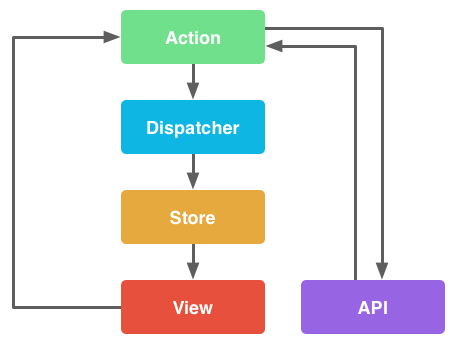
\includegraphics[height=5cm]{figures/react.png}
    \caption{Flux entre les différents composants}
  \end{figure}

  \subsection{Gestion de projet}\label{gestion-de-projet}

  \subsubsection{Relation client}\label{relation-client}

  \bigskip

  Le processus de développement chez Dernier cri se passe généralement
  comme suit. Tout d'abord notre chef de projet, Laetitia Cocusse, discute
  avec le client pour comprendre ses besoins et ses attentes. Selon les
  besoins, elle organise une réunion avec le(s) developpeur(s) et le
  client pour clarifier certains points ou pour discuter des différents
  approches du problèmes possible. C'est l'occasion pour le développeur de
  proposer des solutions, peut être un peu différentes de celles imaginées
  par le client, ou encore de dire son avis sur les prochaines tâches.

  \bigskip

  Ensuite les taches sont estimées par un développeur. Il estime le temps
  qu'il pense passer sur le problème, en prenant en compte l'exploration
  de l'existant, le développement en lui-même, les tests et les possibles
  retours. Cette estimation devra ensuite être validée par le client.

  \bigskip

  Une fois la tache validée, une \emph{issue} est créé dans Github avec
  une description, l'estimation et le développeur à qui est attribuée la
  tache. Cela permet à chacun d'avoir une vue à tout moment de l'évolution
  du projet, des tâches en cours ou terminées. Il est également possible
  de commenter chaque \emph{Issue} pour, par exemple, demander des
  précisions, ou faire remonter une erreur.

  \bigskip

  Selon les priorités, le développeur choisit ou non l'ordre des tâches.
  Pour protéger le projet actuel, stable, des nouvelles modifications tant
  que celles-ci ne sont pas testées, le développeur crée une
  \emph{branche} dans Github, c'est à dire une copie du projet qui
  évoluera indépendamment de la branche principale. C'est sur cette
  branche que seront faites les modifications destinées à implémenter la
  nouvelle fonctionnalité.

  \bigskip

  C'est ensuite le moment de passer au développement à proprement parler.
  Le développeur utilise un environnement de developpement sur son propre
  ordinateur pour simuler l'environnement de production. Cela peut se
  traduire par la création d'une base de données, ou la connexion à une
  \emph{API} spéciale. Il faut faire attention à ce que les données
  utilisée lors de la phase de développement n'aient pas d'impact sur
  celles de production.

  \bigskip

  Quand le développeur estime avoir terminer la tâche, il crée une
  \emph{Pull request} sur Github (comme expliqué plus haut dans le
  rapport). C'est alors le moment de prendre en compte les remarques et
  conseils des autres membres de l'équipe, de corriger éventuellement des
  éléments, pour s'assurer de la qualité du code avant de l'incorporer
  dans le projet.

  \bigskip

  Une fois le développement de la fonctionnalité validé, la nouvelle
  version du site est déployé en \emph{Staging}, c'est à dire une version
  en ligne du site, qui a le même environnement que la production, mais
  avec des fausses données. Ce site sert à tester les nouvelles
  fonctionnalités avant de les pousser sur la production.

  \bigskip

  Laetitia fait une \emph{recette}, c'est à dire vérifie que la version de
  \emph{staging} remplit bien le besoin exprimé par le client, et que la
  nouvelle fonctionnalité n'a pas cassé autre chose. En cas de problème,
  le développeur revient sur la tâche jusqu'à ce que tout soit réglé.

  \bigskip

  Une fois un lot de taches effectuées, il est décidé en accord avec le
  client de pousser les modifications sur la production. Il faut alors
  vérifier que la \emph{mise en prodcution} c'est bien passée : que le
  site fonctionne toujours et que les nouvelles fonctionnalités sont bien
  en place.

  \newpage

  \subsubsection{Organisation interne}\label{organisation-interne}

  \bigskip

  L'entreprise utilise principalement la plateforme Github comme service
  web d'hébergement et donc le logiciel de gestion de versions Git. Github
  est une interface web permettant d'interfacer avec des projets
  versionnés, et composés de multiples applications aidant à la gestion de
  projets.

  \bigskip

  Github propose depuis peu une section \emph{Projet} permettant de gérer
  les \emph{issues}, c'est à dire les tâches. Cette section permet
  notamment de séparer les tâches en plusieures colonnes, par exemple :
  \emph{A faire}, \emph{En cours}, \emph{Terminé}. Il est aussi possible
  d'attribuer les tâches à un contributeur, ou encore de leur attribuer
  des labels tel que \emph{Urgent}, \emph{Bug} ou encore une estimation de
  temps quand à la réalisation de la tâche.

  \bigskip

  Dernier cri utilise ces outils mis à disposition par Github pour mettre
  en place un processus de vérification de la qualité du code et
  d'entraide. Chaque developpeur, une fois une tâche terminée, propose une
  \emph{Pull request}, c'est à dire demande à fusionner sa version du
  projet, modifiée pour résoudre la tâche, avec la version principale,
  stable. Il demande ensuite à ses collégues ayant des compétences dans le
  langage utilisé de relire et de commenter cette \emph{Pull request}.

  \bigskip

  C'est l'occasion pour les développeurs d'avoir l'avis de leurs collégues
  sur leur style d'écriture et leur façon de coder, ce qui permet souvent
  de découvrir de nouvelles méthodes et d'argumenter sur les meilleurs
  techniques à utiliser. Dernier cri utilise ce système de \emph{code
  review} pour garantir une certaine qualité du code ainsi qu'un style
  d'écriture de code homogéne.

  \bigskip

  \section{Mes réalisations}\label{mes-ruxe9alisations}

  \bigskip

  J'ai eu la chance de participer à plusieurs projets durant mon stage, de
  façon plus ou moins importantes. Je vais vous présenter dans cette
  partie les deux principaux projets sur lesquels je me suis investie.

  \bigskip

  J'ai aussi pu travailler sur d'autre projet en renfort sur de courtes
  périodes, ainsi que développer un outils pour le site de Dernier cri.

  \bigskip

  \subsection{Photolix}\label{photolix}

  \subsubsection{Présentation du projet}\label{pruxe9sentation-du-projet}

  \bigskip

  Dès mon arrivée dans l'entreprise j'ai été assigné à la réalisation
  d'une application de développement photo. Le client possède un studio de
  développement photo sur Lille, et souhaitait proposer à sa clientèle un
  site simple et efficace.

  \bigskip

  Le principal objectif de ce projet était de télécharger les photos vers
  le serveur au fur et à mesure de leur sélection, pour ainsi éviter le
  temps d'attente du client à la fin de la saisie de ses informations.

  \bigskip

  Lors de mon arrivée sur le projet, un développeur de Dernier cri avait
  déjà posé des bases. Les fonctions de recadrage et de compression de la
  photo était notamment déjà écrite.

  \bigskip

  \subsubsection{Objectifs}\label{objectifs}

  \bigskip

  Les objectifs du projet Photolix étaient les suivants :

  \begin{itemize}
  \tightlist
  \item
    mettre en place le \emph{design} fournit par le client, à partir des
    maquettes sur Zeplin;
  \item
    gérer l'envoi des photos au serveur;
  \item
    mettre en place la possibilité de modifier les photos (formats,
    orientation\ldots{});
  \item
    pages de saisie des informations du client (adresses, informations de
    paiement) et page de remerciement;
  \end{itemize}

  \bigskip

  \subsubsection{Outils utilisés}\label{outils-utilisuxe9s}

  \bigskip

  Lors de mon arrivée sur ce premier projet, j'ai du apprendre à utiliser
  certains outils, tant au niveau de la gestion de projet, que du
  développement en lui-même.

  \bigskip

  Tout d'abord, le projet utilise Github comme service web d'hébergement
  et de gestion de développement, et par conséquent le logiciel de gestion
  de versions Git. Bien qu'ayant déjà utilisé Git et Github lors de mon
  DUT informatique, de projet personnel ou bien de projet à l'UTC, je ne
  connaissais pas certaines fonctionnalités de Github utilisées par
  l'entreprise, notamment le code review et l'onglet projet. (Voir plus
  haut)

  \bigskip

  Le projet déjà existant utilisait npm comme gestionaire de paquets. npm
  est le gestionnaire de paquets officiel de Node.js. , automatiquement
  installé par défaut depuis la version 0.6.3 de Node.js. npm fonctionne
  avec un terminal et gère les dépendances pour une application. Il permet
  également d'installer des applications Node.js disponibles sur le dépôt
  npm. Il offre également la possibilité de créer des scripts. C'est une
  option vraiment pratique car grace à cela on peut construire et lancer
  l'application en une commande.

  \bigskip

  Pour mon environnement de travail, j'ai aussi utilisé un Linter. Code
  linting est un type d'analyse statique qui est fréquemment utilisé pour
  trouver des modèles problématiques ou le code qui ne respecte pas
  certaines directives de style. Il existe des linters de code pour la
  plupart des langages de programmation, et les compilateurs incorporent
  parfois le linting dans le processus de compilation.

  \bigskip

  J'ai personnellement utilisé ESLint, qui est un utilitaire JavaScript
  open-source et libre créé à l'origine par Nicholas C. Zakas en Juin
  2013. ESLint est écrit en utilisant Node.js pour fournir un
  environnement d'exécution rapide et une installation facile via npm. La
  principale raison pour laquelle ESLint a été créé était de permettre aux
  développeurs de créer leurs propres règles de filtrage.

  \bigskip

  J'ai également pu utiliser le \emph{chatops} de Dernier cri, un outil
  d'administration système via la conversation. Intégré au Slack de
  l'entreprise, il permet à tout le personnel d'obtenir des informations
  sur un serveur ou une application et d'effectuer des résolutions simples
  en cas de panne. Concraitement, j'ai principalement utilisé le chatops
  pour déployer mon application.

  \bigskip

  L'application était écrite en React avec l'utilisation de Redux. J'ai pu
  donc mettre en application les principes appris lors de ma première
  semaine.

  \bigskip

  Pour l'intégration du style du site, j'ai pu utiliser Zeplin. C'est une
  application de collaboration pour les designers et les intégrateurs. Il
  permet aux designers de télécharger leurs maquettes fonctionnelles
  directement à partir de Sketch et les ajouter aux dossiers de projet
  dans Zeplin. Les annotations seront automatiquement ajoutées aux designs
  (tailles, couleurs, marges et même suggestions CSS pour certains
  éléments). Il est alors beaucoup plus simple d'intégrer les maquettes.

  \bigskip

  Finalement, pour l'intégration des maquettes, j'ai fait le choix
  d'utiliser SASS. Sass (Syntactically Awesome Stylesheets) est un langage
  de génération dynamique de feuilles de style. On peut le voir comme une
  extension de CSS3, ajoutant de nouvelles règles dans notre façon
  d'intégrer un web design. Les principaux ajouts sont : les variables,
  les mixins, l'héritage de sélection et différents options très utiles.

  \bigskip

  \subsubsection{Déroulement}\label{duxe9roulement}

  \bigskip

  \paragraph{Intégration des
  maquettes}\label{intuxe9gration-des-maquettes}

  \bigskip

  La première partie du projet consisté à intégrer les maquettes fournit
  par le client. Dans un premier temps, j'ai du redécouper l'application.
  En effet, lors du premier jet réalisé par mon collègue, le client était
  parti sur une application monopage. Mais à la réception des maquettes,
  l'application était devenue multi-page. Il a donc tout d'abord fallut
  mettre en place un routeur pour permettre à l'utilisateur de naviguer
  entre les pages.

  \bigskip

  J'ai choisi, après quelques recherches, d'utiliser React Router.
  \href{https://github.com/ReactTraining/react-router}{React Router} est
  une bibliothèque de routage pour React. Il dispose d'une \emph{API}
  simple avec des fonctionnalités puissantes. Il garde l'interface
  utilisateur synchronisé avec l'\emph{URL}. React Router est très simple
  à utiliser. Il suffit de lister les différentes routes souhaitées,
  associées au composant correspondant.

  \bigskip

  Une fois ce découpage effectué, j'ai mis en place SASS pour la gestion
  des feuilles de style. Pour faciliter son utilisation, j'ai créé
  plusieurs fichiers avec les variables et fonctions (mixins) qui seront
  utilisés dans tout le projet. Le fichier \texttt{variable} contient
  notamment les codes hexadecimaux des couleurs de l'application, les
  tailles des polices d'écriture utilisées, etc. Utiliser des variables
  évite de devoir revenir sur tous les fichiers du projet si l'on décide
  de changer l'une de ses variables.

  \bigskip

  Une fois ces fichiers SASS principaux créés, j'ai simplement créé un
  fichier SASS pour chaque composant React de l'application, qui contient
  donc tout le style de ce composant. J'ai du faire beaucoup de recherches
  pour être à l'aise avec le CSS (Cascading Style Sheets), c'est à dire le
  langage décrivant la présentation de l'application. En effet, jusque là
  je n'avais pas eu l'occasion d'appronfondir mes connaissances en
  intégration.

  \bigskip

  L'intégration du style fut assez rapide, l'application étant
  visuellement assez simple. Grâce à cette première étape j'ai pu me
  familiariser avec l'organisation du projet avant d'attaquer des parties
  plus difficiles.

  \bigskip

  \paragraph{Formatage et téléchargement des
  photos}\label{formatage-et-tuxe9luxe9chargement-des-photos}

  \bigskip

  La deuxième partie du projet était centrée sur le téléchargement des
  photos vers le serveur. Le client a lui même développé une API assez
  simple que nous devions manipuler pour envoyer les photos, changer le
  nombre d'exemplaire, récupérer le prix de la commande\ldots{}

  \bigskip

  La majeur difficulté durant cette étape fut de ne pas avoir accès
  directement à l'API. En effet, celle-ci évoluant en même temps que
  l'application et ne possédant pas de documentation, il était souvent
  nécessaire de demander des précisions ou des évolutions au client. Même
  si la communication était assez rapide, le fait de ne pas avoir la main
  sur l'API a ralenti le développement.

  \bigskip

  Une autre difficulté était le redimensionnement des images avant l'envoi
  au serveur. En effet, quand l'utilisateur sélectionne des photos, nous
  devons tout d'abord passer la photo au format sélectionné, et donc gérer
  les formats incompatibles. Cela a apporté beaucoup de questions. Par
  exemple, si une photo est en 10x15 et que l'utilisateur a sélectionné le
  format 11x15 que fait-on ? Coupe-t-on des morceaux de la photo pour
  arriver au format voulu ? Ou bien ajoute-t-on des bandes ?

  \bigskip

  Cela a donc donné lieu à beaucoup de discutions avec le client pour
  résoudre toutes ses problèmatiques avant de developper les solutions. La
  fonction de redimensionnement est une fonction clé du projet. Une fois
  la photo redimensionnée, nous réduisons la résolution de la photo
  jusqu'a 300dpi (point par pouce). C'est la résolution optimal pour
  l'impression de photo : assez élevée pour garantir une bonne qualité à
  l'impression, et assez faible pour rendre le téléchargement vers le
  serveur le plus rapide possible.

  \bigskip

  \paragraph{Modification des photos}\label{modification-des-photos}

  \bigskip

  L'étape suivante est la création de l'interface et des fonctions
  permettant à l'utilisateur de modifier ses photos. Il peut changer le
  format, recadrer la photo, changer l'orientation\ldots{} J'ai tout
  d'abord chercher s'il existait déja un outil pour le recadrage de la
  photo.

  \bigskip

  C'est à ce moment que j'ai découvert la diversité des outils React
  proposés par la communauté : il est trés facile de trouver des
  composants sur Github qui correspondent à votre besoin. J'ai donc pu
  utiliser
  \href{https://github.com/roadmanfong/react-cropper}{react-cropper},
  trouvé sur Github après quelques recherches, qui s'est révélé très
  efficace. Il permet de gérer le recadrage, fournit des fonctions
  renvoyant toutes les données intéressantes (dimensions du recadrage,
  rotation de la zone de recadrage\ldots{}). Ce fut ma première
  intégration d'un outil React.

  \bigskip

  Pour mettre en place mes autres fonctions de modification des photos,
  j'ai surtout dû modifier la fonction principale de redimensionnement des
  photos, utilisé lors du téléchargement initial. J'y ai ajouté des
  paramétres permettant de choisir le format, l'orientation, si on coupe
  la photo ou bien on ajoute des bandes blanche\ldots{}

  \bigskip

  Enfin, il a fallut mettre en place l'interface utilisateur. Ce fut une
  étape

  \paragraph{Pages informations des clients, paiement et
  remerciement}\label{pages-informations-des-clients-paiement-et-remerciement}

  \bigskip

  La dernière partie du projet consisté à mettre en place les autres pages
  de l'application, servant à récolter les informations nécessaires à la
  commande, et à les envoyer à l'API. Ces pages étaient la page de saisie
  des adresses, de livraison et de facturation, la page de paiement, soit
  par carte bancaire, soit par Paypal, et enfin la page de remerciement
  avec un récapitulatif de la commande, ainsi que des liens pour partager
  l'événement sur les réseaux sociaux.

  \bigskip

  Pour la page de saisie de l'adresse, ce fut l'occasion pour moi de créer
  pour la première fois un formulaire en React et Redux. Avec ce langage,
  la création de formulaire est assez peut instactif car il faut
  répercuter chaque changement des champs, chaque lettre écrite ou
  effacée, pour que l'état de l'applications soit toujours à jour. C'est
  assez fastidieux et inhabituel.

  \bigskip

  Après cette première expériences dans la création de formulaire, j'ai
  pus découvrir un outil, redux-form, permettant de créer beaucoup plus
  facilement des formulaires et gérant automatiquement la mise à jour de
  l'état de l'application. J'ai pu utiliser cet outil dans mon second
  projet. Mais je pense que le fait d'avoir d'abord du faire toute
  l'implémentation nécéssaire par moi même m'a permis de prendre
  conscience des problématiques de cette pile technologique : le maintiens
  de l'état de l'application, la communication entre les
  composants\ldots{}

  \bigskip

  J'ai ensuite travaillé sur le page de remerciement. Sur cette page, on
  affiche un récapitulatif de la commande ainsi que des liens pour
  partager sur les réseaux sociaux l'événement. J'ai ainsi pu apprendre
  comment partager sur Facebook et Tweeter un message, associé a une URL.

  \bigskip

  Finalement, sur les trois pages précédemment citées, j'ai du faire
  apparaitre un récapitulatif de la commande, avec notamment le nombre de
  photos commandé, le prix par photos, le prix total, ainsi que la
  possibilité d'entrer un code de promotion avant le paiement. Cette
  partie à demandé de la réflection car le calculs des prix était
  différent avant et après le paiement. En effet, dans l'absolue, il faut
  récupérer le prix à partir de l'API, pour être certain de son
  exactitude. Cependant, avant le paiement il est possible que toute les
  photos ne soient pas encore envoyé à l'API et donc le pris renvoyé par
  celle-ci n'est pas définitive. IL est alors donc nécéssaire de faire le
  calcul du prix dans l'application, et d'afficher ce resultat dans le
  récapitulatif. Une fois le paiement effectué, il faut afficher le prix
  envoyé par l'API, puisqu'il s'agit du prix final.

  \bigskip

  \paragraph{Fin du projet}\label{fin-du-projet}

  \bigskip

  Vers mi-octobre, j'ai été réaffectée à un autre projet, laissant la fin
  du projet Photolix à Fabien. Il a fini de mettre en place la gestion du
  téléchargement des photos vers le serveur, notamment après leur
  modification. Il a également revu la fonction de redimensionnement des
  photos, car celle utilisée au debut n'était pas assez performante : si
  l'on monté à une centaine de photos chargées, le navigateur ne
  supportait pas la charge.

  \bigskip

  J'ai pu étudier les modifications apportées par Fabien, et apprendre des
  erreurs que j'ai pu commettre. Par exemple, je n'avais pas assez
  travailler la gestion des erreurs. Il a fallut que Fabien reprenne mon
  travail pour ajouter l'affichage des erreurs, en cas par exemple
  d'erreur lors du téléchargement des photos. Ces enseignements m'ont
  permis de ne pas reproduire ces erreurs dans le second projet sur lequel
  j'ai été affecté.

  \bigskip

  Finalement, j'ai pu retravailler sur le projet en decembre. Après un
  premier rendu au client, celui-ci souhaité quelques corrections ainsi
  que l'ajout de quelques fonctionnalités. Il avait utilisé un échantillon
  de client pour tester l'application et avait relevé des améliorations
  possibles à l'interface utilisateur. J'ai donc pu aider Fabien à mettre
  en place ces modifications.

  \bigskip

  \subsubsection{Conclusion}\label{conclusion}

  \bigskip

  Ce premier projet chez Dernier cri m'a beaucoup apporté. Pour commencer,
  j'ai pu me familiariser aves les méthodes de gestion de projet de
  l'entreprise, le processus allant de la formalisation du probléme,
  jusque sa mise en ligne. Dans le même temps j'ai pu prendre en main les
  outils utiliser chez Dernier cri, tel que Github, avec toute la gestion
  des différentes branches, les Pull Request ainsi que la gestion des
  issues\ldots{} Ce fut une étape essenciel pour mon intégration dans
  l'équipe de développement.

  \bigskip

  Ce projet m'a également permit d'apprendre à utiliser React et Redux.
  Ces technologies sont aujourd'hui en pleine expensions, et évolue
  beaucoup et ont un belle avenir devant elles. J'ai également pu
  apprendre a deveopper en front-end, alors que jusque là mes compétences
  techniques étaient plus tournée vers du back.

  \bigskip

  Evidemment, j'ai connus de nombreuse difficultés lors du développemment
  de Photolix. Mon inexpérience m'a conduit à faire des erreurs, à fournir
  un résultat qui n'était pas optimal. J'ai heureusement pu compter sur
  mon collégue, Fabien Gavory, pour me soutenir, me corriger et rattraper
  certaine erreurs, surtout vers la fin du projet. Grace à cela, j'ai pu
  mettre en place de meilleurs pratiques durant le projet suivant.

  \bigskip

  Finalement, c'est une vraie chance d'avoir pu travailler dès mon arrivée
  sur un projet pour un client. J'ai ainsi été tout de suite confrontée
  aux vraie problématiques du developpement d'une application web, de la
  relation cliente, avec des dates butoire et des évolutions des
  spécifications en cours de projet.

  \subsection{Finfrog}\label{finfrog}

  \subsubsection{Présentation du
  projet}\label{pruxe9sentation-du-projet-1}

  \bigskip

  Avec l'arrivée d'un nouveau client et la nécéssité de fournir un
  developpeur React sur ce projet, j'ai quitté le projet Photolix pour
  rejoindre Finfrog.

  \bigskip

  Finfrog est un projet de prêt collaboratif, c'est à dire que le site
  propose des prêt financés par des particuliers. Les prêts proposés vont
  de 200 à 600 euros, à rembourser en 1 à 3 mois. Le but de ce site est
  d'ouvrir, en acceptant des prêts qui ne seraient pas validé par une
  banque car ils sont trop faibles ou bien que la personne est au chômage.

  \bigskip

  Lors de mon arrivée sur le projet, un site été déjà en ligne, développé
  par le client. Le premier objectif était de mettre en place un nouveau
  design sur ce site, d'abord sur la page d'acceuil, et ensuite sur les
  formulaires de demande de prêt.

  \bigskip

  Par la suite, j'ai été amené à developper de nouvelles fonctionnalités
  pour Finfrog, comme la partie du site réservée à la gestion des prêts
  par l'administrateur, les espaces emprunteur et préteur, la génération
  de contrat.

  \subsubsection{Objectifs}\label{objectifs-1}

  \subsubsection{Nouveaux outils}\label{nouveaux-outils}

  \bigskip

  La projet Finfrog utilisait principalement les même outils que Photolix
  : utilisation de npm pour la gestion des paquets, de Zeplin pour étudier
  le design, de React et Redux etc.

  \bigskip

  Cependant à mon arrivée sur FinFrog, le projet était hébergé sur
  Bitbucket et non pas Github. Il a donc fallut que je m'habitue à ce
  nouveaux gestionaire. Par la suite nous avons migré le projet sur
  Github.

  \bigskip

  Sur ce projet, nous avions aussi en charge la partie API et base de
  donnée. L'API est écrite en Nodejs et la base de donnée est une
  postgres, donc manipulable en SQL. Cependant il était rare que je doive
  toucher à la base de donnée.

  \bigskip

  Finalement, pour lancer les processus du site et de l'API, nous avons
  utilisé PM2. PM2 est un gestionnaire de processus de production pour les
  applications Node.js avec un équilibreur de charge intégré. Il vous
  permet de garder les applications en vie pour toujours, de les recharger
  sans temps d'arrêt et de faciliter les tâches administratives courantes
  du système.

  \bigskip

  \subsubsection{Déroulement}\label{duxe9roulement-1}

  \paragraph{Page d'accueil et demande de
  prêt}\label{page-daccueil-et-demande-de-pruxeat}

  \bigskip

  A mon arrivée sur le projet, Dernier cri était chargé de l'intégration
  d'un nouveau design pour le site déjà existant. Cette intégration
  comprenait tout d'abord la page d'accueil, puis le tunnel de demande de
  prêt.

  \bigskip

  \bigskip

  \paragraph{Génération de contrat}\label{guxe9nuxe9ration-de-contrat}

  \bigskip

  \bigskip

  \begin{itemize}
  \item
    Première partie design -\textgreater{} Page d'acceuil : prendre en
    main le projet et ses particuliarité -\textgreater{} Accés restraint
    au debut du projet -\textgreater{} Tunnel emprunteur : on rentre plus
    dans le techniques, la manipulation de redux
  \item
    génération de contrat
  \item
    Grosse passe pour le responsive + cross compatibilité des browsers
  \item
    Communication avec le client ? -\textgreater{} Surtout semaine de noel
    sans Laetitia
  \end{itemize}

  Citer le fait que je n'ai presque pas eu de code review a cause de la
  confidentialité

  \subsubsection{Conclusion}\label{conclusion-1}

  \newpage

  \newpage

  \section{La vie Lilloise}\label{la-vie-lilloise}

  Durant mon stage à Lille j'ai pu me rendre compte que la ville possédait
  une communauté web très active.

  \bigskip

  La ville a notamment reçu le label `French Tech' fin 2014, pour
  récompenser son dynamiste dans le numérique et l'innovation. Ce label,
  en plus de récompenser les efforts de la ville, constitue le point
  d'entrée vers des dispositifs nationaux comme des programmes pour
  attirer les entrepreneurs étrangers qui veulent créer leur
  \emph{start-up} en France.

  \bigskip

  La région profite de la présence de grands groupes nationaux comme
  Orange, Capgemini, IBM France, CGI, CISCO\ldots{}

  \bigskip

  De plus Lille a mis en place un ensemble de structures favorisant
  l'accompagnement et la croissance des startups vers un marché mondial.
  La plus notable est évidemment Euratechnologie, le Pôle d'excellence
  économique dédié aux Technologies de l'Information et de la
  Communication (TIC) de la métropole lilloise. EuraTechnologies a été
  classé dans le top 10 des accélérateurs de \emph{startup} d'Europe par
  Fundacity, et le 1er en France. Euratechnologie posséde des espaces
  dédiés à la recherche, la formation et l'entrepreneuriat, un incubateur
  et un accélérateur.

  \bigskip

  La région lilloise posséde d'autre espaces dédié à l'innovation, les
  \emph{startup} et l'entrepreneuriat : La Plaine Images à Tourcoing et
  Roubaix, Eurasanté à Lille, La Haute Borne à Villeneuve d'Ascq, La Serre
  Numérique à Valenciennes, Le Pôle Numérique Culturel Louvre Lens Vallée
  de Lens\ldots{}

  \bigskip

  La région a connu l'émergence de nombreuse entreprises, prometteuses ou
  déjà fructueuses : Big Ben, Ankama, OVH, Addictiz, Stereograph, Clic \&
  Walk, Giroptic, Mazeberry, Vekia, Sparkow, Mdoloris, A-volute, Critizr,
  Intent Technologies\ldots{}

  \bigskip

  Avoir eu la chance de faire mon stage dans cette région m'a permis de
  profiter de cette écosysteme riche et actif. J'ai pu participer à des
  conférences, des salons et des réunions qui m'ont beaucoup apporté, tant
  au niveau technique que social. Cela m'a permit de préciser mon projet
  professionnel, en m'immergeant dans la vie entreprenariale d'une ville.

  \bigskip

  \subsection{Take Off Conference}\label{take-off-conference}

  \bigskip

  Dernier cri m'a donné l'occasion durant mon stage d'assister à la
  \href{http://takeoffconf.com/2016}{\textbf{Take Off Conference}} les 20
  et 21 octobre 2016. Cet évènement a lieu depuis plusieurs années à
  EuraTechnologies.

  \bigskip

  Historiquement, ce sont les fondateurs de Dernier cri qui ont créé la
  \textbf{Take Off Conference}, avec Florian Le Goff. Aujourd'hui ce sont
  d'autres acteurs de la communauté web de Lille qui ont pris le relais
  pour proposer une nouvelle édition.

  \bigskip

  La \textbf{Take Off Conference} est un cycle de conférences anglophones.
  L'événement dure 2 jours, et accueille des conférenciers du monde
  entier. Bien qu'elle reste avant tout une conférence pour les
  développeurs Web, elle reste accessible pour les développeurs en
  général.

  \bigskip

  Dernier cri m'a permis de participer à cette conférence avec l'un de mes
  collègues. Ce fut une véritable chance pour moi de rencontrer et
  échanger avec des conférenciers du monde entier. Les conférences étaient
  très intéréssantes et inspirantes, sur des sujets très variés allant de
  la compréhension des enjeux de mise en place de nouveau outils, à des
  sujets plus sociaux comme l'acceuil des developpeurs anglais après le
  Brexit.

  \bigskip

  Des évènements ont également été organisé le soir pour permettre aux
  participants et aux conférenciers d'échanger dans un cadre plus détendu.

  \bigskip

  Ce fut une excellente occasion de découvrir de nouvelles technologies,
  de m'ouvrir à des problématiques que je ne connaissais pas ainsi que de
  rencontrer des développeurs qualifiés et passionnés. Lors de ses
  échanges, j'ai pu me rendre compte de la portée internationale de la
  programmation : des personnes des quatres coins du monde se retrouvaient
  sur les mêmes problématiques.

  \bigskip

  \subsection{Meetup}\label{meetup}

  \bigskip

  La communauté web de Lille est très active pour organisé des évenements.
  De très nombreux Meetup sont organisés sur différents domaines du web,
  acceuillant autant des experts que des débutants ou simplement des
  curieux.

  \bigskip

  Très actif dans cette communauté, Dernier cri acceuille au sein de ses
  locaux certaines de ses rencontres. J'ai notamment eu l'occasion
  d'assister à des Meetup de Lille FP (Fonctionnal programming, c'est à
  dire programmation fonctionnelle) et de Lille Elixir.

  \bigskip

  Certains membres de l'équipe sont également investis dans ces
  rencontres, en tant qu'organisateur ou bien speaker. Les patrons les
  poussent à (prendre part a la vie de la communauté web). J'ai ainsi pu
  facilement être au courant des différents évenements Lillois et y
  participer avec mes collégues, ce qui m'a permis d'être bien intégré.

  \bigskip

  \subsection{Maker Faire}\label{maker-faire}

  \bigskip

  La Maker Faire est un autre événement majeur organisé à Lille durant mon
  stage. Ce concept totalement unique regroupe stands de démonstration,
  ateliers de découverte, spectacles et conférences autour des thèmes de
  la créativité, de la fabrication, des cultures Do It Yourself et Makers.

  \bigskip

  Cet événement, présenté par Leroy Merlin en partenariat avec la Ville de
  Lille et lille3000 (programme culturel de la ville de Lille), réunit des
  passionnés de technologies, des artisans, des industriels, des amateurs,
  des ingénieurs, des clubs de science, des artistes, des étudiants et des
  Start'Up. Ils forment la communauté des Makers et viennent pour montrer
  leurs créations, partager leurs connaissances\ldots{}

  \bigskip

  Dernier cri a été invité à assister à la Maker Faire, notamment car nous
  développons l'application web de TechShop, l'atelier collaboratif de
  Leroy Merlin. Dans ce contexte j'ai pu découvrir la communauté
  \emph{Maker} de Lille. J'ai pu notamment décrouvrir les \emph{repair
  coffee}, lieux où l'on peut amener ses appareils électroniques cassés et
  recevoir de l'aide pour leur réparation. Il y avait également des
  robots, des imprimantes 3D, des casques de réalité augmentée \ldots{}
  C'était un endroit plein d'aspiration et d'envie d'entreprendre.

  \newpage

  \section{Conclusion}\label{conclusion-2}

  Ce stage a été très enrichissant pour moi. Il m'a permit de réaliser un
  développement informatique sous la houlette d'une équipe expérimenté,
  qui à su me transmettre des compétences techniques et méthodologiques.

  J'ai aussi pu découvrir la réalité des entreprises et appliquer les
  notions acquises à l'université, apprendre ou de me perfectionner avec
  certaines technologies ou méthodes et de développer l'aptitude au
  travail en équipe.

  Enfin, vous pouvez re-situez votre stage dans votre parcours de
  formation et dans votre projet professionnel. Vos objectifs ont-ils
  évolué ? Par exemple, en quoi ce stage confirme (ou infirme) votre choix
  de filière ?

  -\textgreater{} Compétences apprises : Node React Redux ES6 Relation
  client Git Github pm2 npm

  -\textgreater{} Important : relation client et autonomie, apprentissage
  rapide, equipe disponible et polivalente (qui peut t'aider sur tout)

  -\textgreater{} environnement cool : Ambiance, tech off conf , meetup,
  plus belle vue de Lille

  \newpage

  \section{Glossaire ?}\label{glossaire}

  ES6 React Redux Code review Talk


\end{document}
